\documentclass[11pt,a4paper]{report}

%
% Packages
%
\usepackage[T1]{fontenc}
\usepackage[utf8]{inputenc}
\usepackage{amsmath,amsthm,amssymb}
\usepackage[svgnames]{xcolor}
\usepackage[english,french]{babel}
\usepackage{multicol}
\usepackage{pstricks,pst-node,pst-text,pst-poly,pst-3d}
\usepackage{enumitem}
\usepackage{sidenotes}
\usepackage{graphicx} % Required to insert images
\usepackage{array}
\usepackage{booktabs} % Required for better horizontal rules in tables


%
% Constant and Variables
%
\setlength{\textwidth}{175mm}
\setlength{\textheight}{255mm}
\setlength{\oddsidemargin}{-10mm}
\setlength{\topmargin}{-15mm}
\setlength{\parskip}{0.2cm}

\definecolor{vertfonce}{rgb}{0,0.5,0}

%
% Commands
%
\newcommand{\ds}{\displaystyle}
\newcommand{\scr}{\scriptscriptstyle}
\newcommand{\bs}[1]{\ensuremath{\boldsymbol{#1}}}
\renewcommand{\leq}{\leqslant}
\newenvironment{refer} 
{
	\begin{list}
		{}
		{
			\setlength{\labelwidth}{.5em}
			\setlength{\leftmargin}{0.4cm}
			\setlength{\itemsep}{0cm}
		} 
	}
	{\end{list}}
%\pagenumbering{roman}
%\setcounter{page}{1}

%
\newcounter{num}
\newcommand{\exo}{\addtocounter{num}{1}\noindent{\bf{Exercice \thenum}}\\[-1mm]}
%

%
\newcommand{\donnee}[1]{\\{Donnée: } \emph{#1}}
%


%
% Math
%
\newcommand{\Real}{\mathbb R}
\newcommand{\RPlus}{\Real^{+}}
\newcommand{\norm}[1]{\left\Vert#1\right\Vert}
\newcommand{\abs}[1]{\left\vert#1\right\vert}
\newcommand{\setn}[1]{\left\{#1\right\}_{\scriptscriptstyle n \ge 1}}
\newcommand{\set}[1]{\left\{#1\right\}}
\newcommand{\seq}[1]{\left<#1\right>}
\newcommand{\eps}{\varepsilon}
\newcommand{\To}{\longrightarrow}
\newcommand{\Prob}{\rm{P}}
\newcommand{\F}{\mathcal{F}}
\newcommand{\h}{\mathcal{H}}
\newcommand{\M}{\mathcal{M}}
\newcommand{\N}{\mathcal{N}}
\newcommand{\E}{{\rm E}}
\newcommand{\Hnull}{{\rm H}_{0}}
\newcommand{\Hone}{{\rm H}_{1}}
\newcommand{\Var}{{\rm Var}}
\newcommand{\Cov}{{\rm Cov}}
\newcommand{\sign}{{\rm sign}}
\newcommand{\med}{{\rm med}}
\newcommand{\tr}{{\rm tr}}
\newcommand{\T}{{\text{\tiny \rm T}}}
\newcommand{\minf}{- \, \infty}
\newcommand{\intervalle}[4]{\mathopen{#1}#2\mathpunct{},#3\mathclose{#4}}
\newcommand{\intervalleff}[2]{\intervalle{[}{#1}{#2}{]}}
\newcommand{\intervalleof}[2]{\intervalle{]}{#1}{#2}{]}}
\newcommand{\intervallefo}[2]{\intervalle{[}{#1}{#2}{[}}
\newcommand{\intervalleoo}[2]{\intervalle{]}{#1}{#2}{[}}   
%
\newcommand{\separation}{{\begin{center}\rule{10cm}{0.25pt}\end{center}}\noindent}
%
\frenchspacing


\begin{document}
	\header{variables aléatoires }{Série 3}	
	%
	% Exercice 1
	%
	\begin{exo}
		\donnee{Une boîte contient deux billes noires et trois billes blanches. On tire une bille à la fois, sans remise,
			jusqu’à ce que la première bille noire apparaisse. Dès que la bille noire est tirée, aucune autre bille est
			extraite de la boîte. Désignons par X le nombre de tirages nécessaires. En utilisant un arbre binaire,}
	\end{exo}
	
	%
	% Exercice 2
	%
	\begin{exo}
		\donnee{Des signaux binaires (0 ou 1) sont transmis d’un point A à un point B par un canal de communication. Cependant, une erreur de transmission peut toujours résulter de perturbations aléatoires agissant sur le canal. Supposons qu’un signal émis en A soit correctement enregistré en B avec probabilité 0.8 et ce indépendamment d’un signal à l’autre. Pour essayer d’améliorer la qualité de transmission, on se propose d’émettre chaque signal trois fois de suite, i.e. 000 au lieu de 0 et 111 au lieu de 1.}
	\end{exo}
	%
	% Exercice 3
	%
	\begin{exo}
		\donnee{La fonction de répartition d’une variable aléatoire X est}
	\end{exo}
	
	%
	% Exercice 4
	%
	\begin{exo}
		\donnee{Imaginons qu’on souhaite transmettre les réalisations $x_1, x_2, . . . , x_n$ d’une variable aléatoire discrète X d’un point d’observation A à un point de réception B à l’aide d’un canal de communication ne pouvant transférer que des 0 ou des 1. Ainsi, les valeurs prises par X devront être codées en chaînes formées uniquement de 0 et de 1 avant d’être transmises. Pour éviter toute ambiguïté, on exige qu’un code ne puisse pas être une extension d’un autre.
		\\Comme exemple, supposons que les réalisations de X sont $x_1, x_2, x_3, x_4$. Comme code possible, on peut envisager
		\\$$x_1 \leftrightarrow 00, x_2 \leftrightarrow 01, x_3 \leftrightarrow 10, x_4 \leftrightarrow 11$$Ainsi, si X prend la valeur $x_1$, le message envoyé en B sera 00, il vaudra 01 si X = $x_2$ et ainsi de suite. Un autre code possible est
		\\$$x_1 \leftrightarrow 0, x_2 \leftrightarrow 10, x_3 \leftrightarrow 110, x_4 \leftrightarrow 111$$Un objectif du codage consiste tout naturellement à minimiser le nombre espéré de bits nécessaires pour transmettre l’information. Ainsi, un code est dit plus efficace qu’un autre si son nombre espéré de bits est plus petit que celui nécessaire à l’autre code.}
	\end{exo}
	
	%
	% Exercice 5
	%
	\begin{exo}
		\donnee{Considérons deux variables aléatoires X et Y dont les histogrammes se trouvent dans la figure ci-dessous.\\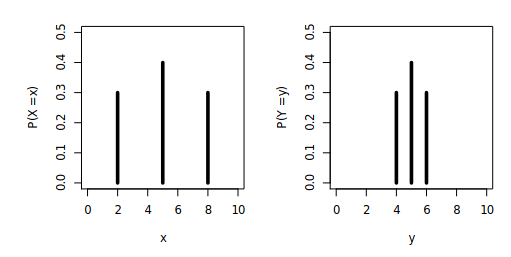
\includegraphics[width=8cm]{ex5.png}
		\\En n’effectuant aucun calcul, l’écart-type de X est-il plus grand que celui de Y ?
		}
	\end{exo}

	%
	% Exercice 6
	%
	\begin{exo}
		\donnee{La distribution de Benford prétend que pour des mesures d’une certaine quantité physique, la probabilité de tomber sur un 1 est de l’ordre de 30 \% alors que celle de tomber sur un 9 est de l’ordre de 4.6 \%. Cette distribution n’est applicable que pour un grand nombre d’objets mesurables. Elle s’applique par exemple aux longueurs de tous les fleuves du monde, aux prix des articles d’un supermarché ou encore aux volumes des tables de logarithmes d’une encyclopédie. En effet, les premières pages de chaque volume sont toujours plus usées que les suivantes, celles du premier volume étant plus utilisées que celles du second et ainsi de suite. Il en sera de même pour les nombres d’une comptabilité. Ainsi, pour détecter d’éventuelles fraudes dans les déclarations d’impôts de grandes entreprises, le fisc américain a utilisé la distribution de Benford. En effet, dans une comptabilité de grande envergure, qui bien souvent est formée de nombreuses pages de chiffres, les comptables essayaient pour déjouer le fisc de créer des données truquées en tirant des nombres au hasard. L’idée n'était pas très bonne. En se livrant à une petite analyse statistique à l’aide de la distribution de Benford, il était possible d’identifier des fraudes dans les déclarations d’impôts de grandes sociétés. La distribution de probabilités de Benford se trouve dans la table ci-dessous.
		\begin{center}
		\begin{tabular}{llllllllll}
			\toprule
			valeur      & 1 	& 2 	& 3 	& 4 	& 5 	& 6 	& 7 	& 8 	& 9 \\
			\midrule
			probabilité & 0.301 & 0.176 & 0.125 & 0.097 & 0.079 & 0.067 & 0.058 & 0.051 &0.046  \\
			\bottomrule
		\end{tabular}
		\end{center}
	}
	\end{exo}
	
	%
	% Footer
	%
	\vfill
	\hrule
	\vspace{2mm}
	\noindent {\tiny Corrigé Etudiant - TIC} \hfill {\tt \tiny \today}
\end{document}
